\documentclass[titlepage]{article}
\usepackage{xeCJK}
\usepackage[top=1.2in, bottom=1.3in, left=1in, right=1in,heightrounded]{geometry}
\usepackage{amsmath}
\usepackage{amsfonts}
\usepackage{graphicx}
\usepackage{tocbibind}
\usepackage{enumitem}
\usepackage{algorithm}
\usepackage{algorithmic}
\usepackage{float}

\renewcommand\refname{参考文献}
\def\NoNumber\#1{{\def\alglinenumber\#\#1{}\State \#1}\addtocounter{ALG@line}{-1}}

\begin{document}
\title{统计自然语言处理基础 \\ 项目报告}
\date{August, 17th 2018}
\author{王巍 \\ \\班号: 1503103 \\ 学号: 1150340114}
\maketitle

\section{分词任务}
\subsection{定义}
中文分词指的是将一个汉字序列切分成一个个单独的词。分词就是将连续的字序列按照一定的规范重新组合成词序列的过程。\cite{definition}
\subsection{实例}
\begin{itemize}
\item 例如一个较为简单的分词任务:
\begin{center}
我国律师工作是随着改革开放和民主法制建设的加强而建立和发展起来的。
\end{center}

\noindent 的分词结果为:
\begin{center}
我国/律师/工作/是/随着/改革/开放/和/民主/法制/建设/的/加强/而/建立/和/发展/起来/的/。\\[2em]
\end{center}

\item 再例如一个由于中文的特性,很可能会被错误分词的例子:
\begin{center}
请把手拿开
\end{center}

\noindent 的分词结果为:
\begin{center}
请把/手/拿开
\end{center}

\noindent 但由于``把手''本身也组成词, 因此也有可能形成错误的分词:
\begin{center}
请/把手/拿开
\end{center}

\item 除此之外,还存在本身具有歧义的句子,比如:
\begin{center}
乒乓球拍卖完了
\end{center}

``乒乓球/拍卖'' 以及`` 乒乓/球拍/卖'' 都是从语法上合理的分词,但语义上的合理性有所不同.
\end{itemize}

\subsection{常用方法}
\begin{itemize}
\item 基于字典匹配的方法\\[1em]
  基于字典匹配的方法又称为机械分词法, 根据扫描的方向和不同长度的匹配情况,可以分为正向最大匹配法,逆向最大匹配法,最少切分以及双向最大匹配法, 在本次项目中, 使用正向最大匹配法结合规则取得了较好的效果, 算法的细节将在下一节讨论.
\item 基于句法的分词方法\\[1em]
  基于句法的分词方法使用计算机模拟人对句子的理解,达到识别词的效果,配合句法语义系统使用. 对于句子本身从语法上没有歧义, 但因为构词而容易产生错误切分的句子,基于句法的分词方法能够较好的解决这种问题. 如上一小节中的第二个例子, 错误的分词方法在语法上存在错误. 但是, 中文的句子构成十分复杂, 句法分析通常难以做到较高的准确率.
\item 基于统计的分词方法\\[1em]
    基于统计的分词方法包括HMM, CRF等, 这类方法将分词视为分类问题, 考察一个字的有限上下文根据统计概率确定其标签, 并通过标签解码出分词结果. 在消除歧义方面, n-gram方法可以在一定程度上解决句子的固有歧义. 如上一小节中的第三个例子, ``乒乓球/拍卖'' 的分词方式出现的频率显然低于`` 乒乓/球拍/卖''的分词方式, 通过这种方法可以选出更为合理的分词. \\

  本次项目中也实现了基于HMM算法的分词, 在没有结合字典,规则, 且训练语料较小的情况下, HMM算法的表现不算很好, 算法的细节也将在下一节中讨论.

\end{itemize}


\section{算法}
\subsection{最大正向匹配算法 (MMSEG)}
\subsubsection{形式化定义}
给定词典$D(w, f)$ ($w$是单词文本, $f$是单词频率). 对于汉字序列$S$, 在$D$上找到所有可能的词块序列$C_{1,2\cdots,n}$ ($C_i=w_1[\_w_2[\_w_3]]$, w是D中的单词). 使得对于算法的词块评分函数$P$, 词块序列的评分之和$\sum_{i=1}^n P(C_i)$之和最大的词块$C_{1,2\cdots,n}^{\max}$即为算法的输出分词方案.
\subsubsection{建模方法}
最大正向匹配算法 (MMSEG)是基于字典匹配的分词方法, 简单高效, 在一定程度上能够解决纯词典方案无法解决的分词歧义问题.\\

\noindent MMSEG算法分为简单算法和复杂算法,其中简单算法对于一个句子,找到其所有的可能前缀; 而复杂算法对于一个句子,前向寻找其可能的``词块'', 即三个或以下个词组, 对可能的词组应用四个启发式规则来解决分歧, 这四个规则即是算法中的词块评分函数,分别是:

\begin{itemize}
\item  备选词块的长度最大:\\[1em]
    例如``长春市长春药店''的分词方案有:
    \begin{itemize}[label=\tiny$\bullet$]
        \item 长春市\_长春\_药店\_
        \item 长春市\_长\_春药\_
        \item 长春\_市长\_春药\_
        \item 长春\_市\_长春\_
        \item 长\_春\_市长\_
    \end{itemize}
    第一种组合长度最长,因此采用第一种分词方案.
\item 备选词组合的平均词长最大:\\[1em]
    例如``国际化''的分词方案有:
    \begin{itemize}
        \item 国际化\_
        \item 国际\_化\_
        \item 国\_际\_化\_
    \end{itemize}
    使用规则1无法过滤,但第一种分词方案的平均长度3为最大, 因此采用第一种分词方案.

\item 备选词组合的变化最小\\[1em]
    例如``北京大学生''的分词方案有:
    \begin{itemize}
        \item 北京大学\_生\_
        \item 北京\_大学生
        \item 北京\_大学\_生\_
        \item 北京\_大\_学生\_
        \item 北\_京\_大学生\_
    \end{itemize}
    经过前两条规则过滤,剩余:
    \begin{itemize}
        \item 北京大学\_生\_
        \item 北京\_大学生
    \end{itemize}
    本条规则在应用中以方差作为度量, 第一种方案方差为1.5, 第二种为0.5. 因此选择第二种方案
\item 备选词组合中,单字词的出现频率统计值最高:
    例如``设施和服务''的分词方案有:
    \begin{itemize}
        \item 设施\_和服\_务\_
        \item 设施\_和\_服务\_
        \item 设\_施\_和服\_
    \end{itemize}
    经前面规则过滤得:
    \begin{itemize}
        \item 设施\_和服\_务\_
        \item 设施\_和\_服务\_
    \end{itemize}
    根据本条规则,显然单字``和''的频率要大于单字``务''的频率, 因此选择第二种方案
\end{itemize}

\noindent 此外, 在实际应用中, 数字和url等的切分需要通过规则来加以约束,具体方案是对数字和url分别用占位符替换, 并备份原数字和url, 在分词结束后进行还原.\\[1em] 

\noindent 基于字典匹配的方法无法正确地识别新词,因此对训练语料或词典的大小有一定的要求,在实验时,也发现随着词典数量的增加,算法在开发集上的准确率会逐步提高, 但使用多个来源不同的词典时, 单词对应的频率将失去意义.

\newpage
\subsubsection{算法伪代码}

\begin{algorithm}
    \renewcommand{\thealgorithm}{}
    \caption{MMSEG-Tokenizer(sentence, dictionary)}
    \begin{algorithmic}[1]
        \REQUIRE chunk has structure with properties corresponding to measurements of 4 rules
        \STATE backups $\leftarrow$ special patterns in sentence
        \STATE replace special patterns in sentence with placeholder
        \STATE words $\leftarrow$ empty list
        \STATE cursor $\leftarrow$ 0
        \REPEAT
        \STATE chunks $\leftarrow$ Get-Chunk(sentence[cursor:])
        \IF{chunks.length > 1}
        \STATE chunks $\leftarrow$ chunk with max total length \COMMENT{rule 1}
        \ENDIF
        \IF{chunks.length > 1}
        \STATE chunks $\leftarrow$ chunk with max average length \COMMENT{rule 2}
        \ENDIF
        \IF{chunks.length > 1}
        \STATE chunks $\leftarrow$ chunk with min standard deviation \COMMENT{rule 3}
        \ENDIF
        \IF{chunks.length > 1}
        \STATE chunks $\leftarrow$ chunk with max single word frequency \COMMENT{rule 4}
        \ENDIF
        \IF{chunks.length > 1}
        \STATE chunks $\leftarrow$ random chunk in chunk \COMMENT{ambiguity cannot be resolved}
        \ENDIF
        
        \STATE cursor $\leftarrow$ cursor + chunks[0].length
        \STATE add chunk to words
        \UNTIL{cursor == length of sentence}
        \STATE result $\leftarrow$ word joined by delimiters
        \STATE restore digits and urls with backups
        RETURN result
    \end{algorithmic}
\end{algorithm}

\begin{algorithm}[H]
    \renewcommand{\thealgorithm}{}
    \caption{Get-Chunk(sentence)}
    \begin{algorithmic}[1]
        \REQUIRE prefix trie already built from dictionary or corpus
        \STATE chunks $\leftarrow$ empty list
        \FOR{$word_1$ in prefixes of sentence}
        \STATE append chunk($word_1$) to chunks
        \FOR{$word_2$ in prefixes of sentence[$word_1.length$:]}
        \STATE append chunk($word_1$, $word_2$) to chunks
        \FOR{$word_3$ in prefixes of sentence[$word_1.length + word_2.length$:]}
        \STATE append chunk($word_1$, $word_2$, $word_3$) to chunks
        \ENDFOR
        \ENDFOR
        \ENDFOR
        \RETURN chunks
    \end{algorithmic}
\end{algorithm}

\subsection{隐马尔科夫模型(HMM)}

\subsubsection{形式化定义}
已知观察序列$Y = (Y_1, Y_2, \cdots, Y_n)$和模型$\theta$, 求解隐藏状态$X = (X_1, X_2, \cdots, X_n)$, 最大化条件概率$P(Y \mathrel| X, \theta)$, 并根绝隐藏状态序列$X$解码得到分词结果.
\subsubsection{建模方法}
HMM模型的参数是一五元组$<StatusSet, ObservedSet, TransProbMatrix, EmitProbMatrix, InitStatus>$组成的, 其中:
\begin{itemize}
    \item StatusSet: 状态值集合,在分词任务中,有四种状态B,M,E,S, 分别表示起始字,中间字,结束字,单字成词.
    \item ObservedSet: 观察值集合,即在训练过程中或预定义的词典中的所有字 
    \item TransProbMatrix: 转移概率矩阵, 马尔科夫链的特点是在$T=i$时刻的状态Status(i),只和$T=i$之前的n个状态有关,HMM中假设n=1, 因此在这里状态转移矩阵是一个4*4的矩阵,分别对应前一个状态的BMES到下一个状态的BMES的转移概率.
    \item EmitProbMatrix: 发射概率矩阵, 发射概率是一个条件概率, 对观察值i和状态j, 发射概率表示为$P(Observed[i]\mathrel|Status[j])$, 由观察值独立性假设, 有:
$$
P(Observed[i], Status[j]) = P(Status[j]) * P(Observed[i]\mathrel|Status[j])
$$
    \item InitStatus: 初始状态分布, 即各个作为第一个字出现的概率分布, 显然, 状态M和S的初始概率为0
\end{itemize}
HMM模型求解中文分词问题的核心在于求解隐藏状态序列的Viterbi\cite{viterbi}算法, 该算法通过动态规划的方式求解状态转移图上概率最大的路径.

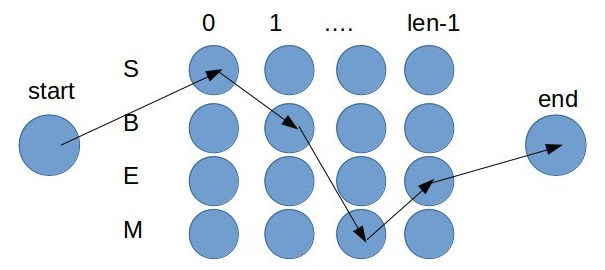
\includegraphics[width=0.8\textwidth]{viterbi.png}

\newpage
\subsubsection{算法伪代码}
训练HMM模型的过程虽然代码冗长,但实际上只是简单的对训练语料的概率统计的过程,因此在算法部分,主要说明Viterbi算法的伪代码

\begin{algorithm}[H]
    \renewcommand{\thealgorithm}{}
    \caption{Viterbi(obs)}
    \begin{algorithmic}[1]
        \STATE probs $\leftarrow$ empty list of dictionary
        \STATE path $\leftarrow$ emtpy dictionary
        \FOR{state in StatusSet} 
        \STATE probs[0][state] $\leftarrow$ $P(state\mathrel|obs[0])$
        \STATE add state to path
        \ENDFOR
        \FOR{$i=1$ to $obs.length$}
        \STATE new-path $\leftarrow$ empty list of dictionary
        \FOR{state in StatusSet}
        \STATE from-state $\leftarrow$ $argmax_{state}$ $P(prev-state) * P(state\mathrel|prev-state) * P(obs[i]\mathrel|state)$
        \STATE new-path $\leftarrow$ path[from-state] concat state
        \ENDFOR
        \STATE update path with new-path
        \ENDFOR
        \RETURN path with largest probs
    \end{algorithmic}
\end{algorithm}
\section{实验结果}
\subsection{数据规模}
\begin{itemize}
    \item 训练数据:\\[1em]
        使用ir.hit.edu.cn提供的训练语料, 包含7000行, 185815个词, 20941个不重复的词, 此外MMSEG方法使用清华大学开发语料库``诗词'',``成语'',``地名''词库作为补充.\\
    \item 测试数据:\\[1em]
        使用ir.hit.edu.cn提供的开发语料, 其中语料1包含1000行, 26853个词, 6889个不重复的词; 语料2包含201行, 7402个词, 2392个不重复的词.
\end{itemize}
\subsection{评价方法}
评价方法使用ir.hit.edu.cn提供的eval.py, 使用权重相等的准确率和召回率的综合性能指标 $F1-measure$
其中准确率Precision:
$$
Precision = \frac{\texttt{正确切分的词数}}{\texttt{切分出词的总数}}
$$
召回率Recall:
$$
Recall = \frac{\texttt{正确切分的词数}}{\texttt{应切分出词的总数}}
$$
评价指标:
$$
f_1 = \frac{2 * Precision * Recall}{Precision + Recall}
$$
\subsection{准确率}
\subsubsection{MMSEG}
\begin{itemize}
    \item 开发语料1:\\[1em]
        \#recall 24573\\
        \#gold 26853\\
        \#predict 28650\\
        f: 0.884168423328
    \item 开发语料2:\\[1em]
        \#recall 6328\\
        \#gold 7402\\
        \#predict 8186\\
        f: 0.811906594817
\end{itemize}
\subsubsection{HMM}
\begin{itemize}
    \item 开发语料1:\\[1em]
        \#recall 21520\\
        \#gold 26853\\
        \#predict 27029\\
        f: 0.798782524776
    \item 开发语料2:\\[1em]
        \#recall 5066\\
        \#gold 7402\\
        \#predict 6962\\
        f: 0.70537454748
\end{itemize}
\begin{thebibliography}{1}

    \bibitem{definition} https://baike.baidu.com/ 中文分词

    \bibitem{MMSEG} Chih-Hao Tsai \textit{A Word Identification System for Mandarin Chinese Text Based on Two Variants of the Maximum Matching Algorithm} http://technology.chtsai.org/mmseg/ 

    \bibitem{viterbi} P.Antal \textit{Hidden Markov Models} antal@mit.bme.hu

\end{thebibliography}
\end{document}
